\documentclass[12pt, letterpaper]{article}
\usepackage[margin=0.5in]{geometry}
\usepackage{amsmath}
\usepackage{amssymb}
\usepackage{mathabx}
% \usepackage{minted}
\usepackage{graphicx}
% \graphicspath{ {./images/} }

\usepackage{fancybox}
\setlength\parindent{0pt}

\title{Assignment 4}
\author{Lokesh Mohanty (SR no: 21014)}
\date{November 2022}

\begin{document}
\fontsize{14pt}{18pt}\selectfont

\maketitle

\section*{Problem 1}
\label{sec:prob1}

\subsection*{Procedure:}
\begin{itemize}
\item Choose 1st column, find the row with the max element and swap the whole row with the 1st row.
  
\item Make this max element the pivot. Divide the 1st row by the pivot. Since this divides the value of the determinant by the pivot, store this value so that we can multiply the final value of determinant with this.
  
\item Make every element below it in the column $0$ by subtracting the current element times the 1st row from the current row (doesn't change the determinant).
  
\item Repeat the above 3 steps for the sub-matrix(i.e., the matrix excluding the 1st column and 1st row)
  
\item Store the total number of swaps across all the loops (i.e., the number of times the max element is not in the 1st row of the sub-matrix) as this multiplies the determinant by $-1$.
  
\item After the whole iteration, the matrix is reduced to an upper triangular matrix with all diagonal elements as 1 whose determinant is 1.
  
\item Hence the determinant of the matrix will be the product of all the pivots multiplied with $(-1)$ to the power of number of swaps.
\end{itemize}

\subsection*{Number of Flops} 
\begin{itemize}
\item Division by pivot: $n + (n-1) + (n-2) + ... + 1 = \frac{n(n-1)}{2}$
  
\item making below elements $0$: $2(n-1)^2 + 2(n-2)^2 + ... + 2(1)^2 = \frac{n(n-1)(2n-1)}{3}$
  
\item finding determinant (product of pivots): n
  
\item \textbf{Total}: $n + \frac{n^2 - n}{2} + \frac{2n^3 - 3n^2 + n}{3}
  = \frac{2}{3}n^3 - \frac{1}{2}n^2 + \frac{5}{6}n$
\end{itemize}


\pagebreak
\section*{Problem 2}
\label{sec:prob2}

\begin{verbatim}
  import numpy as np
  from scipy.linalg import lu
  import matplotlib.pyplot as plt
  from random import random

  # LU decomposition without partial pivoting
  def customLU(A):
      n = A.shape[0]
      L = np.identity(n)
      U = A

      for i in range(n - 1):
          for j in range(i + 1, n):
              L[j, i] = U[j, i] / U[i, i]
              U[j, i:] = U[j, i:] - L[j,i] * U[i, i:]

      return L, U

  error = []
  error_custom = []
  for N in range(5, 21):
      A = [random() for _ in range (N)]
      A = A - np.diag(A) + np.diag(0.001 * np.ones((N, 1)))

      # LU decomposition with partial pivoting
      P, L, U = lu(A)
      error.append(np.linalg.norm(A - P.dot(L).dot(U)))

      # LU decomposition without partial pivoting
      L, U = customLU(A)
      error_custom.append(np.linalg.norm(A - L.dot(U)))


  fig, ax = plt.subplots(2, 1)
  ax[0].plot(range(5, 21), error, label="partial pivot", marker="v")
  ax[0].plot(range(5, 21), error_custom, label="without partial pivot", marker="x")
  ax[0].legend(loc="upper left")
  ax[0].set_title("With vs Without partial pivot")
  ax[0].set_xlabel("N")
  ax[0].set_ylabel("Frobenius norm error")

  ax[1].plot(range(5, 21), error, label="partial pivot", marker="v")
  ax[1].legend(loc="upper left")
  ax[1].set_title("With partial pivot")
  ax[1].set_xlabel("N")
  ax[1].set_ylabel("Frobenius norm error")

  plt.savefig("2.png")
\end{verbatim}

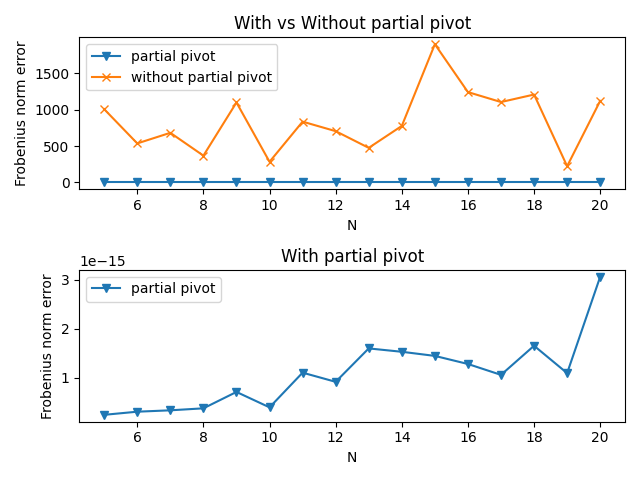
\includegraphics{2}

\pagebreak
\section*{Problem 3}
\label{sec:prob3}

\paragraph{(a)} 

We know that for a unique Cholesky factorization to exist, the matrix should be symmetric positive definite (SPD).\\

We know that a non-singular square matrix $\mathbf{A}$ has an SVD(singular value decomposition) with all non-zero real singular values. And since the singular values of $\mathbf{A}$ are the square root of eigenvalues of $\mathbf{A}^T\mathbf{A}$, we can say that $\mathbf{A}^T\mathbf{A}$ is SPD(symmetric-positive definite) and hence has a unique cholesky factorization.

\begin{align*}
  \mathbf{A}^T\mathbf{A} = \mathbf{U}^T\mathbf{U} \\
  \implies \mathbf{R}^T\mathbf{Q}^T\mathbf{Q}\mathbf{R} = \mathbf{U}^T\mathbf{U} \\
  \implies \mathbf{R}^T\mathbf{R} = \mathbf{U}^T\mathbf{U}
\end{align*}

Since the cholesky factorization is unique, $\mathbf{R} = \mathbf{U}$.

Hence Proved.

\paragraph{(b)}
Let $\mathbf{\Phi} = \begin{pmatrix} \phi_1(x) & \phi_2(x) & ... & \phi_m(x) \end{pmatrix}$
and $\mathbf{\Phi}' = \begin{pmatrix} \frac{d\phi_1(x)}{dx} & \frac{d\phi_2(x)}{dx} & ... & \frac{d\phi_m(x)}{dx} \end{pmatrix}$
\begin{align*}
  \implies \int_{-1}^1 \phi_i(x)\phi_j(x)dx &= \mathbf{\Phi}^T\mathbf{\Phi}\\
  \text{and}&\\
  \implies \int_{-1}^1 \frac{d\phi_i(x)}{dx}\frac{d\phi_j(x)}{dx}dx &= \mathbf{\Phi'}^T\mathbf{\Phi'}\\
\end{align*}

As proved earlier since $\mathbf{\Phi}$ and $\mathbf{\Phi}'$ are non-singular square matrices, $\mathbf{\Phi}^T\mathbf{\Phi}$ and  $\mathbf{\Phi}'^T\mathbf{\Phi'}$ are symmetric positive definite matrix

\paragraph{(c)}

We know that if there exists a matrix $\mathbf{B}$ such that $\mathbf{A} = \mathbf{B}^T\mathbf{B}$ then $\mathbf{A}$ is symmetric, positive definite as we have already proved in part \textbf{(a)}.\\

And since we know that for a symmetric, strictly positive definite matrix $\mathbf{A}$ the cholesky factorization exists and is unique, we can write $\mathbf{A} = \mathbf{B}^T\mathbf{B}$ where $\mathbf{B} \in \mathbb{R}^{m \times n}$ and is a full rank matrix.

\pagebreak
\section*{Problem 4}
\label{sec:prob4}

\paragraph{(a)} $\lambda$ is an eigenvalue of $\mathbf{A}$ and $\mu \in \mathbb{C}$.

\paragraph{Proof:}
As per the definition of eigenvalue, eigenvector, ($\mathbf{v}$ is the corresponding eigen vector of $\lambda$)
\begin{align*}
  \implies \mathbf{A}\mathbf{v} &= \lambda \mathbf{v} \\
  \implies \mathbf{A}\mathbf{v} - \mu \mathbf{v}
                                &= \lambda \mathbf{v} - \mu \mathbf{v} \\
  \implies (\mathbf{A} - \mu \mathbf{I})\mathbf{v} &= (\lambda - \mu)\mathbf{v} \\
\end{align*}

This implies that $\lambda - \mu$ is an eigenvalue of $\mathbf{A} - \mu \mathbf{I}$ with the same eigen vector $\mathbf{v}$

\paragraph{(b)} If $\mathbf{A}$ is real and $\lambda$ is an eigenvalue of $\mathbf{A}$, then $-\lambda$ need not be an eigenvalue of $\mathbf{A}$

\paragraph{Counter Example:} Let $\mathbf{A} = \mathbf{I} = \begin{pmatrix} 1 & 0 \\ 0 & 1 \end{pmatrix}$,

 Here we can see that the eigenvalues of $\mathbf{A}$ are both $1$ and $-1$ is not an eigenvalue of $\mathbf{A}$. Hence proved.

\paragraph{(c)} If $\mathbf{A}$ is real and $\lambda$ is an eigenvalue of $\mathbf{A}$ then $\lambda^{*}$ is also an eigenvalue of $\mathbf{A}$

\paragraph{Proof:}
As per the definition of eigenvalue, eigenvector, ($\mathbf{v}$ is the corresponding eigen vector of $\lambda$)
\begin{align*}
  \implies \mathbf{A}\mathbf{v} &= \lambda \mathbf{v} \\
  &\text{Taking Conjugate on both sides} \\
  \implies (\mathbf{A}\mathbf{v})^{*} &= (\lambda \mathbf{v})^{*} \\
  \implies \mathbf{A}^{*}\mathbf{v}^{*} &= \lambda^{*} \mathbf{v}^{*} \\
  &\text{Since $\mathbf{A}$ is real, $\mathbf{A}^{*} = \mathbf{A}$} \\
  \implies \mathbf{A}\mathbf{v}^{*} &= \lambda^{*} \mathbf{v}^{*} \\
\end{align*}

This implies that $\lambda^{*}$ is also an eigenvalue of $\mathbf{A}$. Hence proved.

\paragraph{(d)} If $\lambda$ is an eigen value of $\mathbf{A}$ and $\mathbf{A}$ is non-singular, then $\lambda^{-1}$ is the eigenvalue of $\mathbf{A}^{-1}$

\paragraph{Proof:}
As per the definition of eigenvalue, eigenvector, ($\mathbf{v}$ is the corresponding eigen vector of $\lambda$)
\begin{align*}
  \implies \mathbf{A}\mathbf{v} &= \lambda \mathbf{v} \\
  &\text{Multiplying $\mathbf{A}^{-1}$ as $\mathbf{A}$ is non-singular} \\
  \implies (\mathbf{A}^{-1}\mathbf{A}\mathbf{v}) &= (\lambda \mathbf{A}^{-1}\mathbf{v}) \\
  \implies \mathbf{v} &= \lambda \mathbf{A}^{-1}\mathbf{v} \\
  \implies \lambda \mathbf{A}^{-1}\mathbf{v} &= \mathbf{v} \\
  \implies \mathbf{A}^{-1}\mathbf{v} &= \lambda^{-1} \mathbf{v} \\
\end{align*}

This implies that $\lambda^{-1}$ is also an eigenvalue of $\mathbf{A}$. Hence proved.

\paragraph{(e)} If all the eigenvalues of $\mathbf{A}$ are zero, then $\mathbf{A} \not = 0$

\paragraph{Counter Example:} Let $\mathbf{A} =
\begin{pmatrix} 0 & 0 \\ 2 & 0 \end{pmatrix}$, i.e., any triangular matrix with all diagonal elements as zero.

The above matrix has the characteristic equation: $\lambda^2 = 0$ i.e., all the eigenvalues are zero but the matrix is not a zero matrix. Hence proved.

\paragraph{(f)} If $\mathbf{A}$ is diagonalizable and all its eigenvalues are equal, then $\mathbf{A}$ is diagonal.

\paragraph{Proof:}

Since $\mathbf{A}$ is diagonalizable, algebraic multiplicity = geometric multiplicity and since all the eigenvalues are equal, $\mathbf{A}$ is a matrix with equal number of rows and columns (i.e., square matrix).

We can choose eigenvectors that are orthogonal to each other and are normalized such that $\mathbf{A}\mathbf{v}_i = \lambda_i \mathbf{v}_i$. Considering all the eigenvectors, the equation can be formulated in terms of $\mathbf{A}, \mathbf{V}, \mathbf{\Lambda}$ where $\mathbf{V}$ is the collection of all eigenvectors as its columns and hence is orthogonal and $\mathbf{\Lambda}$ is the collection of all respective eigenvalues and hence is diagonal.
\begin{align*}
  \implies \mathbf{A}\mathbf{V} &= \mathbf{\Lambda} \mathbf{V} \\
  &\text{Multiply $\mathbf{V}^T$ on both sides} \\
  \implies \mathbf{A}\mathbf{V}\mathbf{V}^T &= \mathbf{\Lambda} \mathbf{V}\mathbf{V}^T \\
  &\text{Since \textbf{V} is orthogonal, $\mathbf{V}\mathbf{V}^T$ is \textbf{I}} \\
  \implies \mathbf{A}\mathbf{I} &= \mathbf{\Lambda} \mathbf{I} \\
  \implies \mathbf{A} &= \mathbf{\Lambda} \\
\end{align*}

This implies that $\mathbf{A}$ is a diagonal matrix. Hence proved.

\pagebreak
\section*{Problem 5}
\label{sec:prob5}

\paragraph{(a)} Every eigenvalue of $\mathbf{A}$ lies in a Greshgorin disk.

\paragraph{Proof:}
Let $\mathbf{A}\mathbf{v} = \lambda \mathbf{v}$ with max element in $\mathbf{v}$ as 1.

\begin{align*}
  \implies \sum_{i,j}^n A_{i, j}v_j &= \lambda v_i, \forall i \\
  \implies \sum_{i,j}^n A_{i, j}v_j &= \lambda v_i, \forall i \\
  \implies (\lambda - A_{i,i})v_i &= A_{i,1}v_1 + A_{i,2}v_2 + ... + 0 + ... + A_{i,n}v_n, \forall i \\
  \implies |(\lambda - A_{i,i})v_i| &\leq |A_{i,1}v_1| + |A_{i,2}v_2| + ... + 0 + ... + |A_{i,n}v_n|, \forall i \\
  &\leq |A_{i,1}v_i| + |A_{i,2}v_i| + ... + 0 + ... + |A_{i,n}v_i|, \forall i \\
  &= (|A_{i,1}| + |A_{i,2}| + ... + 0 + ... + |A_{i,n}|)|v_{max}|, \forall i \\
  &\text{since we choose \textbf{v} such that max element in $\mathbf{v}$ is 1}
  &= (|A_{i,1}| + |A_{i,2}| + ... + 0 + ... + |A_{i,n}|), \forall i \\
  \implies |(\lambda - A_{i,i})| &\leq (|A_{i,1}| + |A_{i,2}| + ... + 0 + ... + |A_{i,n}|), \forall i \\
  \implies |(\lambda - A_{i,i})| &\leq r_i, \forall i \\
\end{align*}

Hence Proved.

\paragraph{(b)} Given that $|a_{ii}| > r_i$

But from \textbf{(a)} we know that $|a_{ii} - \lambda| \leq r_i$. But for $\mathbf{A}$ to be singular, there should exist a $\lambda$ such that $\lambda = 0$ i.e., $|a_{ii} - 0| \leq r_i$ but since $|a_{ii}| > r_i$, it is a contradiction. Hence $\mathbf{A}$ can't be singular. Threrefore $\mathbf{A}$ is invertible.

\paragraph{(c)} $\mathbf{A} =
\begin{bmatrix} 
  8 & 2 & 0 \\ 1 & 4 & \epsilon \\ 0 & \epsilon & 1
\end{bmatrix}$\\

\begin{align*}
  a_{11} = 8 , r_1 = 2 \implies |\lambda - 8| &\leq 2
  \implies \lambda \leq 10 \text{ or } \lambda \geq 6 \\
  a_{22} = 4 , r_2 = 1 + \epsilon  \implies |\lambda - 4| &\leq 1 + \epsilon
  \implies \lambda \leq 5 + \epsilon \text{ or } \lambda \geq 3 - \epsilon \\
  a_{33} = 1 , r_3 = \epsilon  \implies |\lambda - 1| &\leq \epsilon
  \implies \lambda \leq 1 + \epsilon \text{ or } \lambda \geq 1 - \epsilon \\
\end{align*}

Therefore, the estimates for eigen values are:
\begin{itemize}
\item Maximum: 10
\item Minimum: $\geq 1 - \epsilon \approx 0$
\end{itemize}

\end{document}

%%% Local Variables:
%%% mode: latex
%%% TeX-master: t
%%% End:
